
\section{Supplementary material for Chapter 1}
\label{supp:chapter1}

\vspace*{1cm}

\subsection{Supplementary Appendix A: Insights on the
models}
\label{chap1:appendixA}


%\setcounter{figure}{0}
%\setcounter{table}{0}

%\pagenumbering{arabic}
%\renewcommand*{\thepage}{A--\arabic{page}}

\begin{figure}[htbp]
\centering 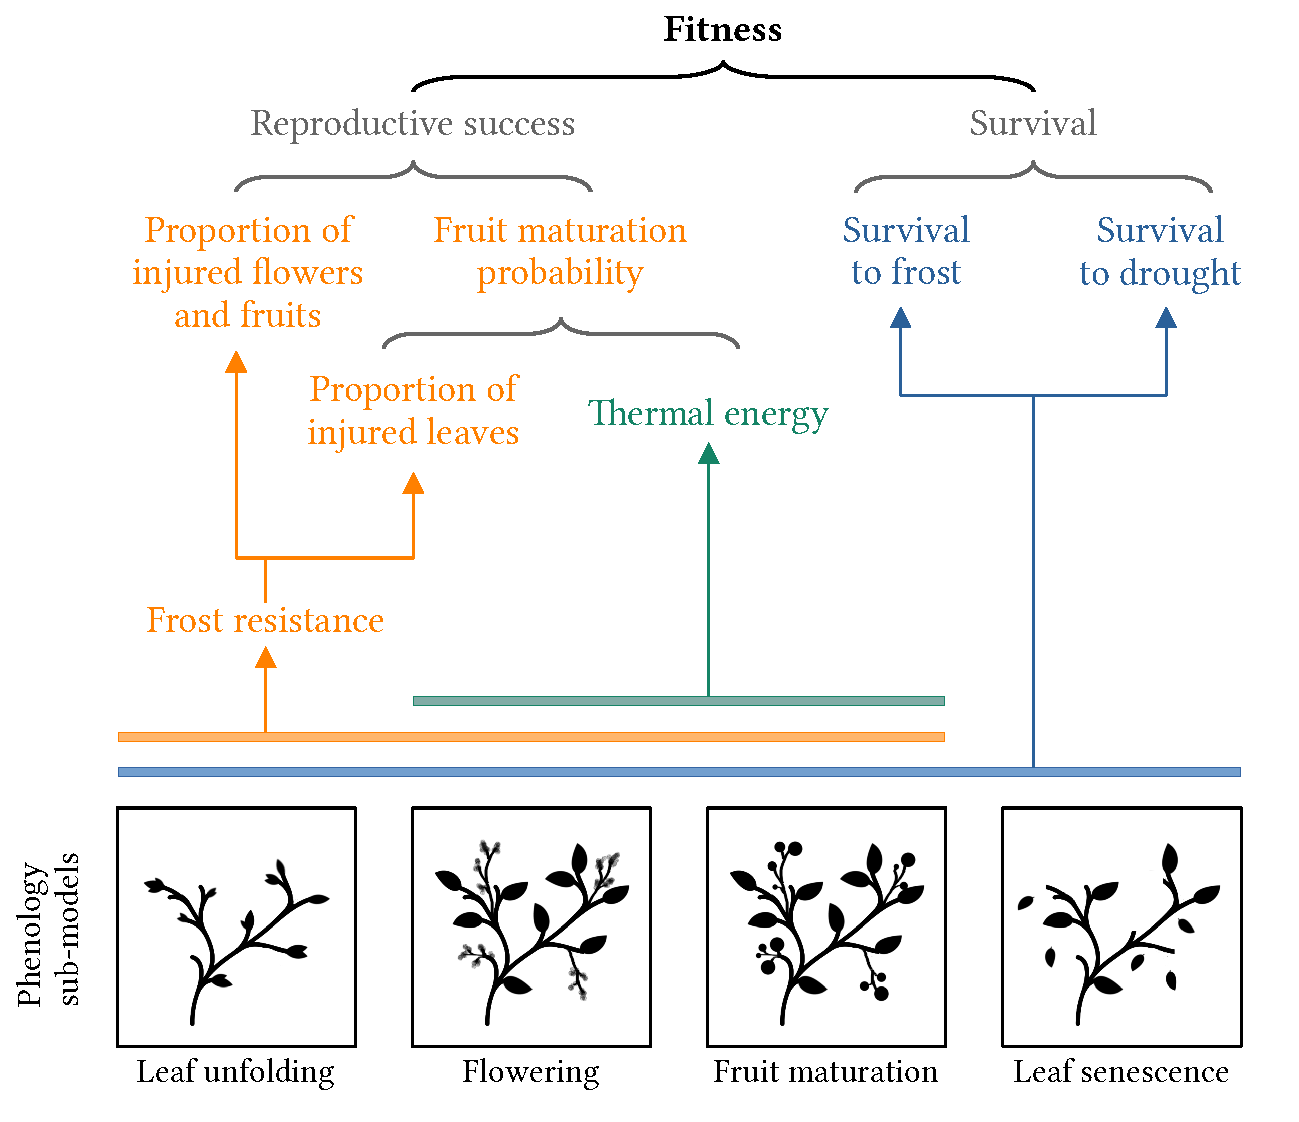
\includegraphics{chapter1/figs/supp/phenofit} 
\caption{PHENOFIT model in a nutshell.}\label{figS:phenofit_model}
\end{figure}

\begin{figure}[htbp]
\centering 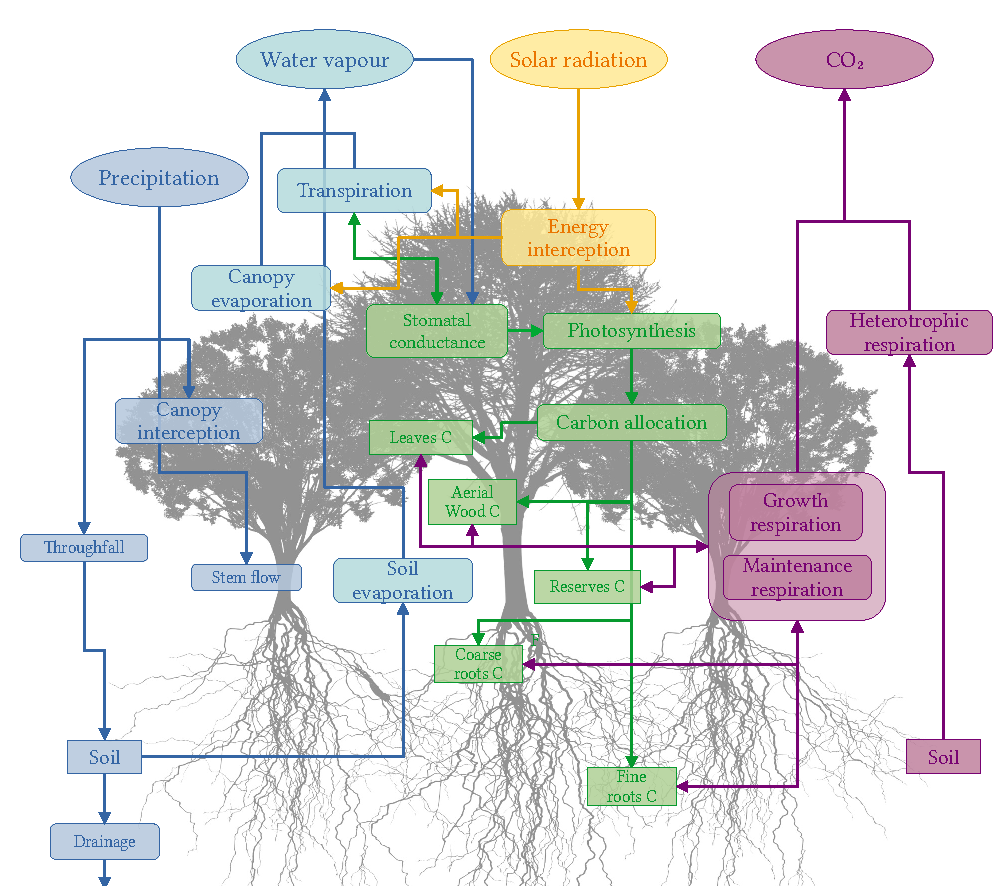
\includegraphics{chapter1/figs/supp/castanea_schema}
\caption{CASTANEA model in a nutshell.}\label{figS:castanea_model}
\end{figure}

\newpage

\subsection{Supplementary Appendix B: Processing of occurrence
data}\label{chap1:appendixB}

%\renewcommand*\thetable{B.\arabic{table}}
%\renewcommand*\thefigure{B.\arabic{figure}}

%\setcounter{figure}{0}
%\setcounter{table}{0}

%\pagenumbering{arabic}
%\renewcommand*{\thepage}{B--\arabic{page}}

%\hfill \break

\begin{table}[!h]

\caption{\label{tab:unnamed-chunk-1}GBIF download links}
\centering
\begin{tabular}[t]{ccc}
\toprule
Species & Number of occurrences & Download link\\
\midrule
Fagus sylvatica & 718.898 & https://doi.org/10.15468/dl.e9wasa\\
Quercus ilex & 78.979 & https://doi.org/10.15468/dl.2a4haw\\
Abies alba & 119.891 & https://doi.org/10.15468/dl.my6c9t\\
\bottomrule
\end{tabular}
\end{table}

\hfill \break

\begin{figure}[htbp]
\centering 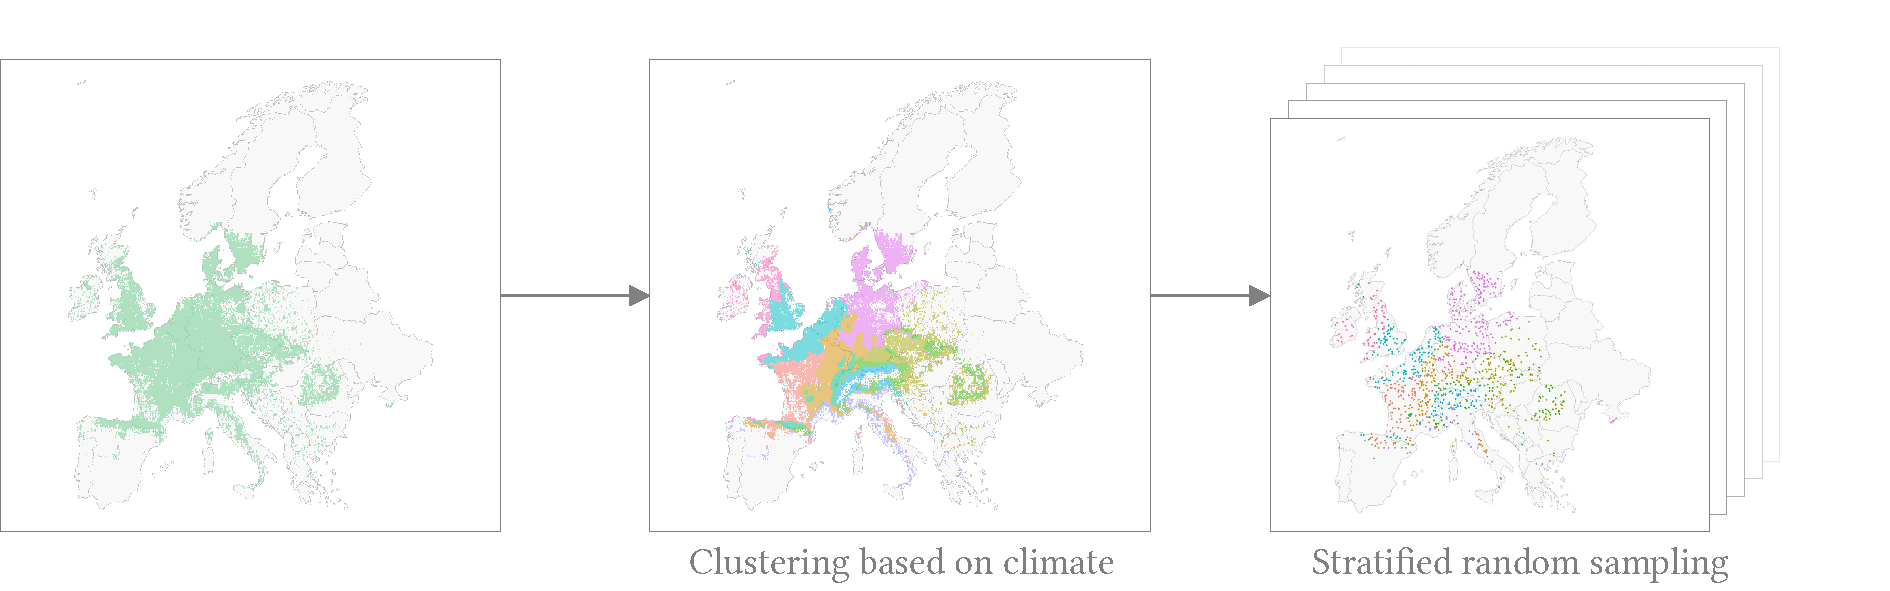
\includegraphics{chapter1/figs/supp/presence_clustering} 
\caption{Stratified random sampling of beech presence records based on climate clusters.}\label{fig:pres_clustering}
\end{figure}

\begin{landscape}
\begin{figure}[htbp]
\centering 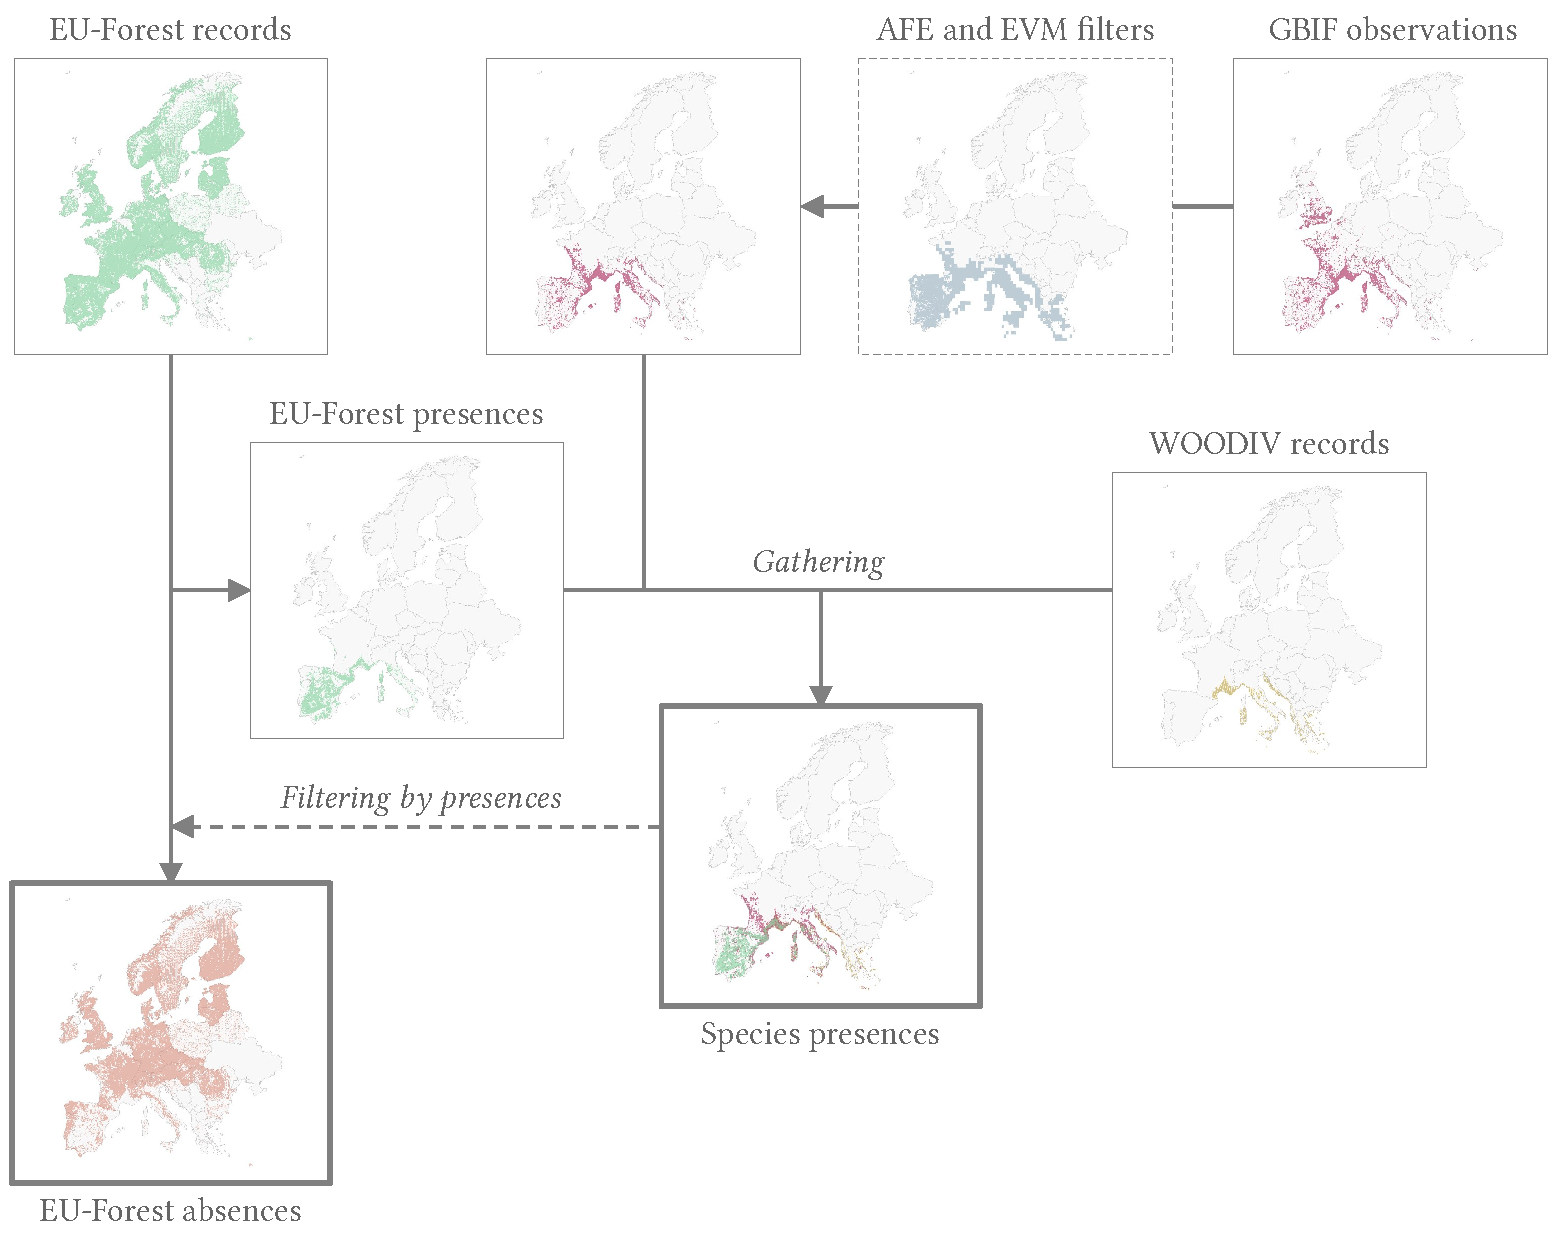
\includegraphics{chapter1/figs/supp/occurrence_processing} 
\caption{Processing of holm oak occurrence records. GBIF: Global Biodiversity Information Facility, AFE: Atlas Flora Europeae, EVM: EuroVegMap.}\label{fig:occ_processing}
\end{figure}
\end{landscape}

\newpage

\newpage

\subsection{Supplementary Appendix C: Species
distributions}\label{chap1:appendixC}
\vspace*{3cm}

%\renewcommand*\thetable{C.\arabic{table}}
%\renewcommand*\thefigure{C.\arabic{figure}}

%\setcounter{figure}{0}
%\setcounter{table}{0}

%\pagenumbering{arabic}
%\renewcommand*{\thepage}{C--\arabic{page}}

\begin{figure}
\vspace*{-2cm}
\centering
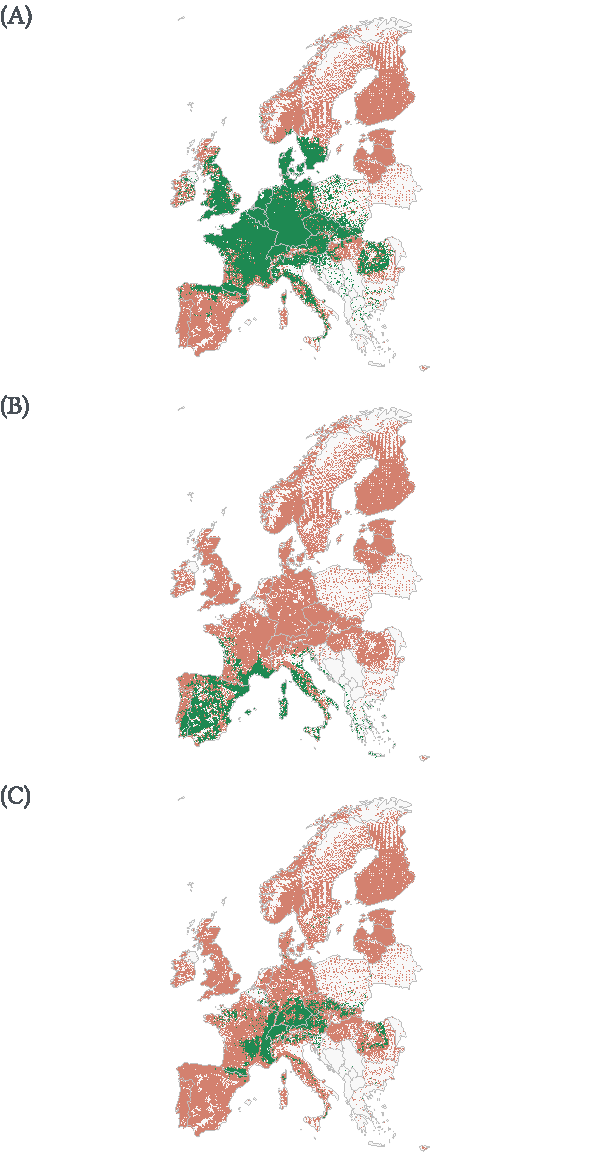
\includegraphics{chapter1/figs/supp/distributionmaps.pdf}
\caption{Species distributions of \textbf{(A)} beech, \textbf{(B)} holm
oak and \textbf{(C)} silver fir. Green cells are \(0.1^\circ\) cells
where species is present, orange cells where species is supposed to be
absent.}
\end{figure}

\newpage

\subsection{Supplementary Appendix D: Objective function and constraint
handling in CMA-ES}\label{chap1:appendixD}

%\renewcommand*\thetable{D.\arabic{table}}
%\renewcommand*\thefigure{D.\arabic{figure}}

%\setcounter{figure}{0}
%\setcounter{table}{0}

%\pagenumbering{arabic}
%\renewcommand*{\thepage}{D--\arabic{page}}

%\hfill \break

\subsubsection{The AUC as an objective
function}\label{the-auc-as-an-objective-function}

The AUC is the area under the receiver operating characteristic curve,
which plots sensitivity (correctly predicted positive fraction) as a
function of commission error (falsely predicted positive fraction), as
the probability threshold discriminating presence/absence varies. It is
a discrimination metric, which has been widely used in the species
distribution modelling literature.

\subsubsection{Box constraint handling}\label{box-constraint-handling}

With this constraint handling - implemented by default in the R package
\emph{cmaes} (\protect\hyperlink{ref-Trautmann2011}{Trautmann \emph{et
al.} 2011}) - each evaluated solution is guaranteed to lie within the
feasible space. Let's say we have a parameter vector \(x\). For each
parameter \(x_i\), we have a lower bound \(lb_i\) and an upper bound
\(ub_i\). If a parameter \(x_i\) violates one of this bound, we set
\(x_i\) to a new value \(x_i^{repaired}\) equal to the closest boundary
value (\(lb_i\) or \(ub_i\)). We thus obtained a new parameter set
\(x^{repaired}\), with a minimal \(\|x-x^{repaired}\|\) value. This new
feasible solution \(x^{repaired}\) is used for the evaluation of the
objective function \(AUC_{model}(x^{repaired})\), and to compute a
penalty term
\(pen=\sum\limits_{i}(x_i-x_i^{repaired})^2=\|x^{repaired}-x\|^2\). Then
\(x^{repaired}\) is discarded, and the algorithm computes the penalized
objective function of \(x^{repaired}\) as follows:
\(AUC_{model}(x)=AUC_{model}(x^{repaired})+pen\). This boundary handling
could be improved with adaptive weights (see
\protect\hyperlink{ref-Hansen2009}{Hansen \emph{et al.} 2009}).

\subsubsection{Ecological infeasibility
constraint}\label{ecological-infeasibility-constraint}

We added a simple way to handle ecological constraint (e.g.~unfolding
before flowering in beech mixed bud) with a death penalty. When a
parameter vector \(x\) violates a constraint, it is rejected and
generated again. The main drawback of this approach is that CMA-ES does
not use information from unfeasible points. An other approach could be
to set \(AUC_{model}(x)=0\). However, as our feasible space was large,
the death penalty constraint worked well in our case.

We applied an inequality constraint on both \textit{Fagus sylvatica} and
\textit{Quercus ilex}, which have mixed buds (leaves and flowers within
the same bud): unfolding must happen before flowering. On the contrary,
we did not apply any inequality constraint on \textit{Abies alba} simple
bud phenology parameters.

\newpage

\subsection{Supplementary Appendix E: Holm oak and silver fir
calibrations}\label{chap1:appendixE}

%\renewcommand*\thetable{E.\arabic{table}}
%\renewcommand*\thefigure{E.\arabic{figure}}

%\setcounter{figure}{0}
%\setcounter{table}{0}

%\pagenumbering{arabic}
%\renewcommand*{\thepage}{E--\arabic{page}}

\begin{figure}[H]
\centering 
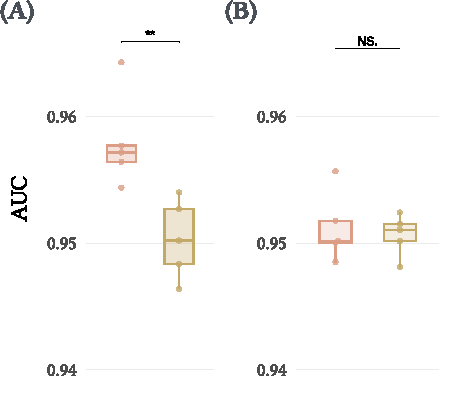
\includegraphics{chapter1/figs/supp/calibCMAESquercus} 
\caption{CMA-ES calibration using the PHENOFIT model and holm oak: \textbf{(A)} calibration AUC (only calibration cells) and \textbf{(B)} total AUC (every presence/absence cells). Each color is a different sub-sampling of occurrence data, each point is a calibration run. The black horizontal bars represent the pairwise Mann–Whitney tests between the two subsets.}\label{fig:calibCMAESquercus}
\end{figure}

\begin{figure}[H]
\centering 
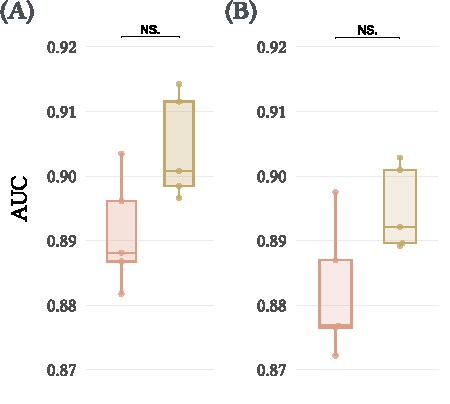
\includegraphics{chapter1/figs/supp/calibCMAESabies} 
\caption{CMA-ES calibration using the PHENOFIT model and silver fir: \textbf{(A)} calibration AUC (only calibration cells) and \textbf{(B)} total AUC (every presence/absence cells). Each color is a different sub-sampling of occurrence data, each point is a calibration run. The black horizontal bars represent the pairwise Mann–Whitney tests between the two subsets.}\label{fig:calibCMAESabies}
\end{figure}

\newpage

\subsection{Supplementary Appendix F: Raw model outputs}\label{chap1:appendixF}

%\renewcommand*\thetable{F.\arabic{table}}
%\renewcommand*\thefigure{F.\arabic{figure}}

%\setcounter{figure}{0}
%\setcounter{table}{0}

%\pagenumbering{arabic}
%\renewcommand*{\thepage}{F--\arabic{page}}

%\hfill \break


\begin{figure}[ht!]
\centering 
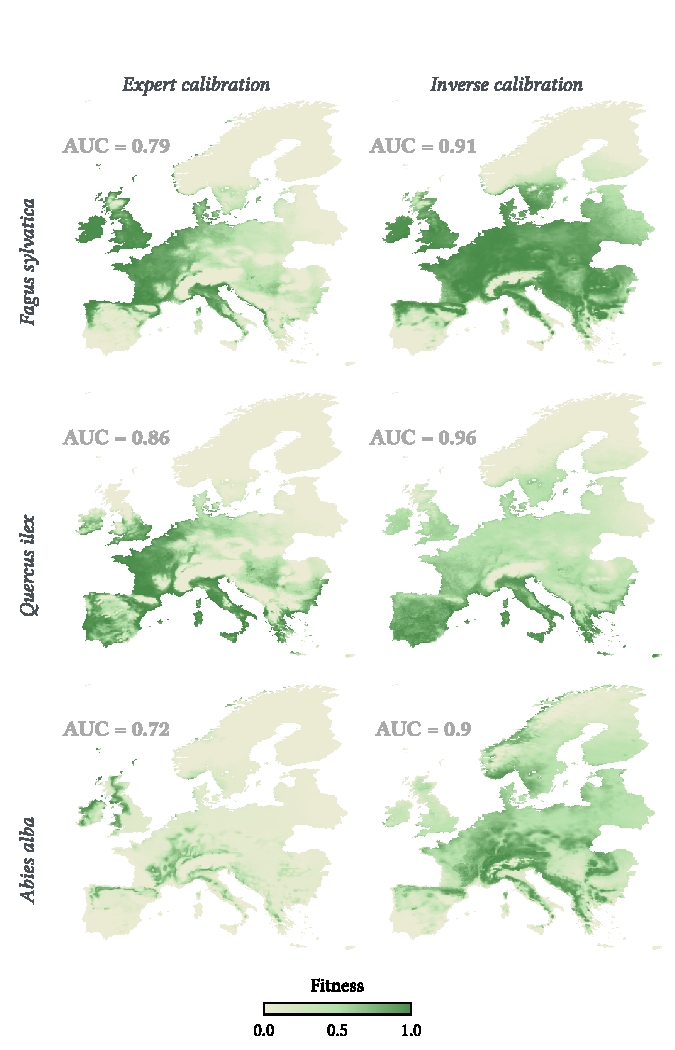
\includegraphics{chapter1/figs/supp/phenofit_output_maps}
\caption{Fitness index predicted by PHENOFIT with the expert and the inverse calibrations.}\label{fig:phenofit_output_maps}
\end{figure}

\newpage

\begin{figure}[H]
\centering 
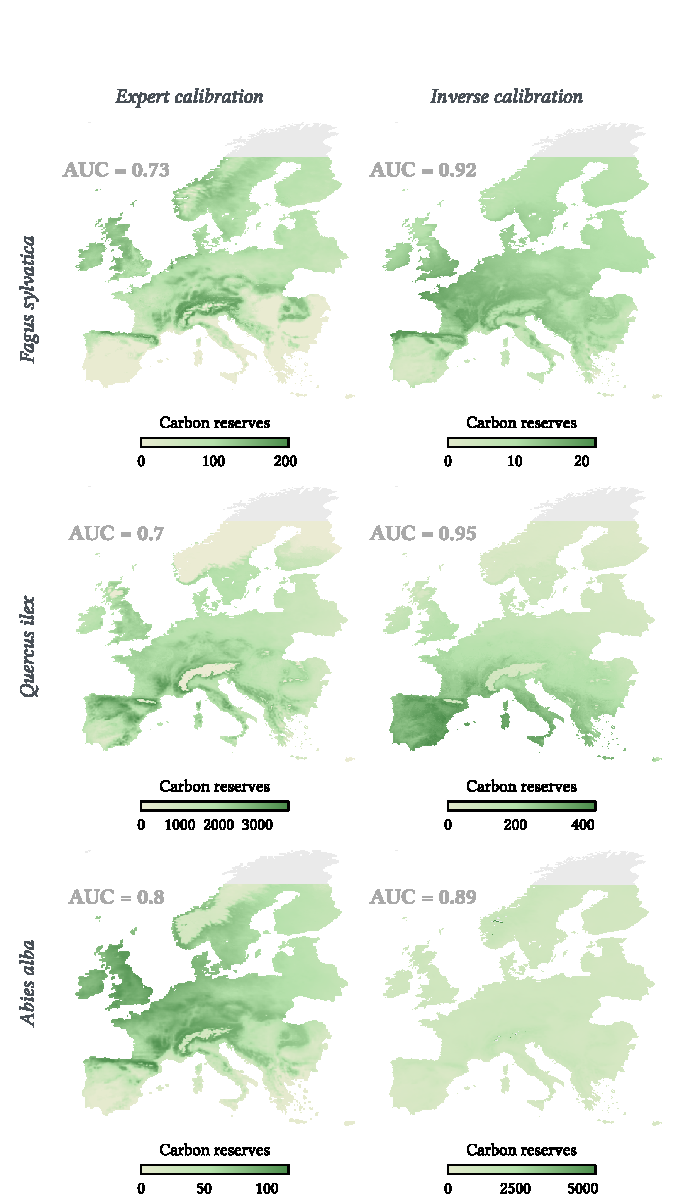
\includegraphics{chapter1/figs/supp/best_forward_maps} 
\caption{Carbon reserves predicted by CASTANEA with the expert and the inverse calibrations. Note that CASTANEA cannot be used in high-latitude regions (grey area).}\label{fig:best_forward_maps}
\end{figure}


\vspace*{3cm}

\subsection{Supplementary Appendix G: Leaf unfolding
submodel}\label{chap1:appendixG}

%\renewcommand*\thetable{G.\arabic{table}}
%\renewcommand*\thefigure{G.\arabic{figure}}

%\setcounter{figure}{0}
%\setcounter{table}{0}

%\pagenumbering{arabic}
%\renewcommand*{\thepage}{G--\arabic{page}}

%\hfill \break

\subsubsection{Fagus sylvatica leaf unfolding
submodel}\label{fagus-sylvatica-leaf-unfolding-submodel}

This model, called UniChill (\protect\hyperlink{ref-Chuine2000}{Chuine
2000}), is a sequential two-phase model (endodormancy and ecodormancy
phases).\\
The endodormancy phase begins at day \(t_0\). The daily rate of chilling
\(R_c\) is defined as a threshold function of the daily mean temperature
\(T_d\): \[ R_c(T_d) = \left\{
\begin{array}{ll}
      0 & T_d \geq T_b \\
      1 & T_d < T_b \\
\end{array} 
\right. \] where \(T_b\) is the threshold temperature below which the
bud accumulates chilling units.\\
The endodormancy releases at day \(t_c\) when the accumulated rate of
chilling has reached the level \(C_{crit}\):
\[\sum\limits_{t_0}^{t_c} R_c(T_d) \geq C_{crit} \] Then, the
ecodormancy phase begins. The daily rate of forcing \(R_f\) is defined
as a sigmoid function of the daily mean temperature \(T_d\):
\[R_f(T_d) = \frac{1}{1 + e^{-d_T(T_d-T_{50})}} \] where \(d_T\) is the
slope and \(T_{50}\) the mid-response temperature. Bud break occurs at
day \(t_f\) when the accumulated rate of forcing has reached the level
\(F_{crit}\): \[\sum\limits_{t_c}^{t_f} R_f(T_d) \geq F_{crit} \] Thus,
the UniChill model has 6 parameters: \(t_0\), \(T_b\) and \(C_{crit}\)
for the first phase, \(d_T\), \(T_{50}\) and \(F_{crit}\) for the second
phase.

\begin{figure}[h]
\centering 
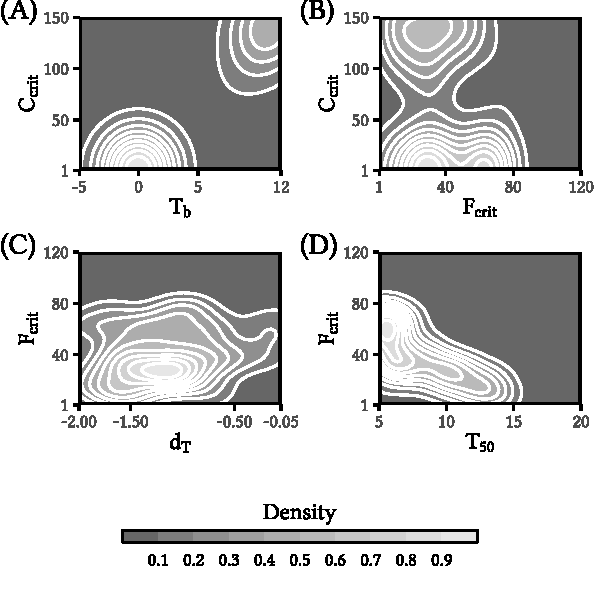
\includegraphics{chapter1/figs/supp/leafpardensity} 
\caption{Beech leaf unfolding model parameter density. Y-axis and X-axis limits are lower and upper bounds used during calibration.}\label{fig:leafpardensity}
\end{figure}

\begin{figure}[h]
\centering 
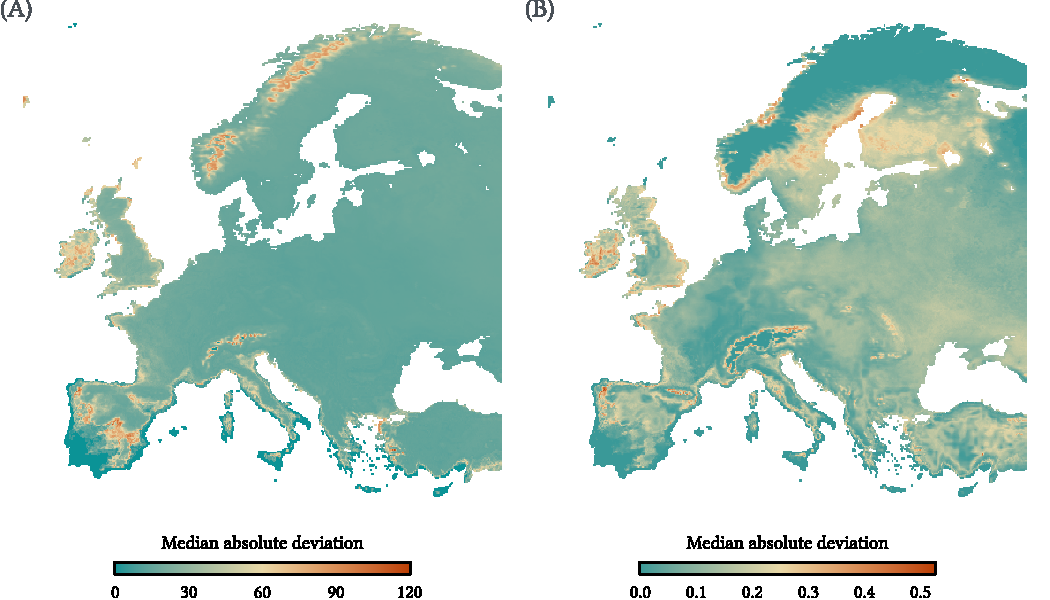
\includegraphics{chapter1/figs/supp/consensusfitnessmap} 
\caption{Median absolute deviation of beech \textbf{(A)} leaf unfolding date and \textbf{(B)} fitness, predicted with 100 calibrated parameter sets of PHENOFIT.}\label{fig:consensusfitnessmap}
\end{figure}

The median standard deviation of unfolding date across Europe was about
15.4 days. On beech presence points, it was about 16.2 days. Nearly
90.3\% of cells had a median absolute deviation lower than 30 days
(\hyperref[fig:consensusfitnessmap]{Figure F.2.A.}). The median standard
deviation of fitness across Europe was about 0.148. On beech presence
points, it was about 0.153. Nearly 46.4\% and 91.5\% of total cells had
a median absolute deviation lower than 0.1 and 0.2 respectively
(\hyperref[fig:consensusfitnessmap]{Figure F.2.B.}).

\begin{figure}[h]
\centering 
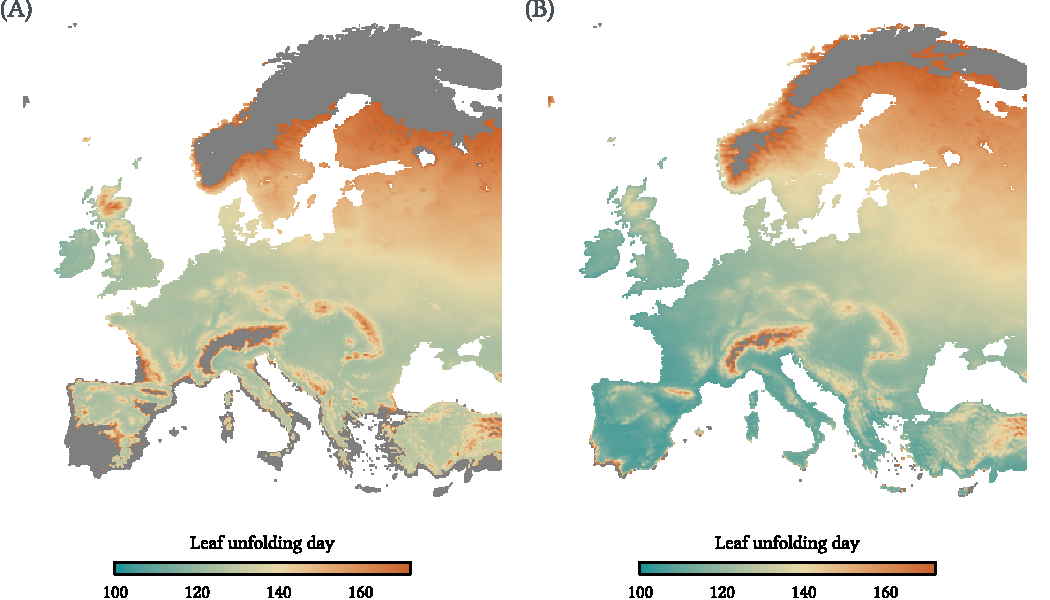
\includegraphics{chapter1/figs/supp/unfoldingdatesbackforw} 
\caption{Mean leaf unfolding day of beech with \textbf{(A)} best CMA-ES calibrated parameters and \textbf{(B)} expert parameters. Values above June solstice day (167) are in grey. Note that PHENOFIT model assign a value of 365 when unfolding has not happened at all due to climate conditions.}\label{fig:unfoldingdatesbackforw}
\end{figure}